\documentclass{article}

  % packages
    % basic stuff for rendering math
    \usepackage[letterpaper, top=1in, bottom=1in, left=1in, right=1in]{geometry}
    \usepackage[utf8]{inputenc}
    \usepackage[english]{babel}
    \usepackage{amsmath} 
    \usepackage{amssymb}
    % \usepackage{amsthm}

    % extra math symbols and utilities
    \usepackage{mathtools}        % for extra stuff like \coloneqq
    \usepackage{mathrsfs}         % for extra stuff like \mathsrc{}
    \usepackage{centernot}        % for the centernot arrow 
    \usepackage{bm}               % for better boldsymbol/mathbf 
    \usepackage{enumitem}         % better control over enumerate, itemize
    \usepackage{hyperref}         % for hypertext linking
    \usepackage{fancyvrb}          % for better verbatim environments
    \usepackage{newverbs}         % for texttt{}
    \usepackage{xcolor}           % for colored text 
    \usepackage{listings}         % to include code
    \usepackage{lstautogobble}    % helper package for code
    \usepackage{parcolumns}       % for side by side columns for two column code
    

    % page layout
    \usepackage{fancyhdr}         % for headers and footers 
    \usepackage{lastpage}         % to include last page number in footer 
    \usepackage{parskip}          % for no indentation and space between paragraphs    
    \usepackage[T1]{fontenc}      % to include \textbackslash
    \usepackage{footnote}
    \usepackage{etoolbox}

    % for custom environments
    \usepackage{tcolorbox}        % for better colored boxes in custom environments
    \tcbuselibrary{breakable}     % to allow tcolorboxes to break across pages

    % figures
    \usepackage{pgfplots}
    \pgfplotsset{compat=1.18}
    \usepackage{float}            % for [H] figure placement
    \usepackage{tikz}
    \usepackage{tikz-cd}
    \usepackage{circuitikz}
    \usetikzlibrary{arrows}
    \usetikzlibrary{positioning}
    \usetikzlibrary{calc}
    \usepackage{graphicx}
    \usepackage{caption} 
    \usepackage{subcaption}
    \captionsetup{font=small}

    % for tabular stuff 
    \usepackage{dcolumn}

    \usepackage[nottoc]{tocbibind}
    \pdfsuppresswarningpagegroup=1
    \hfuzz=5.002pt                % ignore overfull hbox badness warnings below this limit

  % New and replaced operators
    \DeclareMathOperator{\Tr}{Tr}
    \DeclareMathOperator{\Sym}{Sym}
    \DeclareMathOperator{\Span}{span}
    \DeclareMathOperator{\std}{std}
    \DeclareMathOperator{\Cov}{Cov}
    \DeclareMathOperator{\Var}{Var}
    \DeclareMathOperator{\Corr}{Corr}
    \DeclareMathOperator{\pos}{pos}
    \DeclareMathOperator*{\argmin}{\arg\!\min}
    \DeclareMathOperator*{\argmax}{\arg\!\max}
    \newcommand{\qed}{\hfill$\blacksquare$}     % I like QED squares to be black

  % Custom Environments
    \newtcolorbox[auto counter, number within=section]{question}[1][]
    {
      colframe = orange!25,
      colback  = orange!10,
      coltitle = orange!20!black,  
      breakable, 
      title = \textbf{Question \thetcbcounter ~(#1)}
    }

    \newtcolorbox[auto counter, number within=section]{exercise}[1][]
    {
      colframe = teal!25,
      colback  = teal!10,
      coltitle = teal!20!black,  
      breakable, 
      title = \textbf{Exercise \thetcbcounter ~(#1)}
    }
    \newtcolorbox[auto counter, number within=section]{solution}[1][]
    {
      colframe = violet!25,
      colback  = violet!10,
      coltitle = violet!20!black,  
      breakable, 
      title = \textbf{Solution \thetcbcounter}
    }
    \newtcolorbox[auto counter, number within=section]{lemma}[1][]
    {
      colframe = red!25,
      colback  = red!10,
      coltitle = red!20!black,  
      breakable, 
      title = \textbf{Lemma \thetcbcounter ~(#1)}
    }
    \newtcolorbox[auto counter, number within=section]{theorem}[1][]
    {
      colframe = red!25,
      colback  = red!10,
      coltitle = red!20!black,  
      breakable, 
      title = \textbf{Theorem \thetcbcounter ~(#1)}
    } 
    \newtcolorbox[auto counter, number within=section]{corollary}[1][]
    {
      colframe = red!25,
      colback  = red!10,
      coltitle = red!20!black,  
      breakable, 
      title = \textbf{Corollary \thetcbcounter ~(#1)}
    } 
    \newtcolorbox[auto counter, number within=section]{proof}[1][]
    {
      colframe = orange!25,
      colback  = orange!10,
      coltitle = orange!20!black,  
      breakable, 
      title = \textbf{Proof. }
    } 
    \newtcolorbox[auto counter, number within=section]{definition}[1][]
    {
      colframe = yellow!25,
      colback  = yellow!10,
      coltitle = yellow!20!black,  
      breakable, 
      title = \textbf{Definition \thetcbcounter ~(#1)}
    } 
    \newtcolorbox[auto counter, number within=section]{example}[1][]
    {
      colframe = blue!25,
      colback  = blue!10,
      coltitle = blue!20!black,  
      breakable, 
      title = \textbf{Example \thetcbcounter ~(#1)}
    } 
    \newtcolorbox[auto counter, number within=section]{code}[1][]
    {
      colframe = green!25,
      colback  = green!10,
      coltitle = green!20!black,  
      breakable, 
      title = \textbf{Code \thetcbcounter ~(#1)}
    } 

    \BeforeBeginEnvironment{example}{\savenotes}
    \AfterEndEnvironment{example}{\spewnotes}
    \BeforeBeginEnvironment{lemma}{\savenotes}
    \AfterEndEnvironment{lemma}{\spewnotes}
    \BeforeBeginEnvironment{theorem}{\savenotes}
    \AfterEndEnvironment{theorem}{\spewnotes}
    \BeforeBeginEnvironment{corollary}{\savenotes}
    \AfterEndEnvironment{corollary}{\spewnotes}
    \BeforeBeginEnvironment{definition}{\savenotes}
    \AfterEndEnvironment{definition}{\spewnotes}
    \BeforeBeginEnvironment{exercise}{\savenotes}
    \AfterEndEnvironment{exercise}{\spewnotes}
    \BeforeBeginEnvironment{proof}{\savenotes}
    \AfterEndEnvironment{proof}{\spewnotes}
    \BeforeBeginEnvironment{solution}{\savenotes}
    \AfterEndEnvironment{solution}{\spewnotes}
    \BeforeBeginEnvironment{question}{\savenotes}
    \AfterEndEnvironment{question}{\spewnotes}
    \BeforeBeginEnvironment{code}{\savenotes}
    \AfterEndEnvironment{code}{\spewnotes}

    \definecolor{dkgreen}{rgb}{0,0.6,0}
    \definecolor{gray}{rgb}{0.5,0.5,0.5}
    \definecolor{mauve}{rgb}{0.58,0,0.82}
    \definecolor{lightgray}{gray}{0.93}

    % default options for listings (for code)
    \lstset{
      autogobble,
      frame=ltbr,
      language=C,                           % the language of the code
      aboveskip=3mm,
      belowskip=3mm,
      showstringspaces=false,
      columns=fullflexible,
      keepspaces=true,
      basicstyle={\small\ttfamily},
      numbers=left,
      firstnumber=1,                        % start line number at 1
      numberstyle=\tiny\color{gray},
      keywordstyle=\color{blue},
      commentstyle=\color{dkgreen},
      stringstyle=\color{mauve},
      backgroundcolor=\color{lightgray}, 
      breaklines=true,                      % break lines
      breakatwhitespace=true,
      tabsize=3, 
      xleftmargin=2em, 
      framexleftmargin=1.5em, 
      stepnumber=1
    }

  % Page style
    \pagestyle{fancy}
    \fancyhead[L]{Information Theory, Signal Processing}
    \fancyhead[C]{Muchang Bahng}
    \fancyhead[R]{Spring 2024} 
    \fancyfoot[C]{\thepage / \pageref{LastPage}}
    \renewcommand{\footrulewidth}{0.4pt}          % the footer line should be 0.4pt wide
    \renewcommand{\thispagestyle}[1]{}  % needed to include headers in title page

\begin{document}

\title{Information Theory and Signal Processing} 
\author{Muchang Bahng}
\date{Spring 2024}

\maketitle
\tableofcontents
\pagebreak

\section{Introduction}

  \subsection{Channels}

    In a \textit{communication system}, we have a \textit{transmitter} and \textit{receiver}, with \textit{signals} going through a \textit{channel}. Let's briefly define what these terms are, which are pretty much taken verbatim from Shannon's famous paper \cite{shannon}. 

    \begin{figure}[H]
      \centering 
      \includegraphics[scale=0.35]{img/channel_diagram.png}
      \caption{A channel diagram. } 
      \label{fig:channel_diagram}
    \end{figure}

    \begin{definition}[Information Source]
      An \textbf{information source} produces a message or sequence of messages to be communicated to the receiving terminal.  
    \end{definition}

    \begin{definition}[Encoder]
      A \textbf{transmitter}, or \textbf{encoder}, operator on the message in some way to produce a signal suitable for transmission over the channel. 
    \end{definition}

    \begin{definition}[Channel]
      The \textbf{channel} is the medium used to transmit the signal from the encoder to the decoder. Some examples of channels are: 
      \begin{enumerate}
        \item A copper wire is a channel connecting one phone to another phone. 
        \item Air is a channel connecting your voice to another's ear. 
        \item Vacuum is a channel connecting an antenna on earth to the Mars rover.  
      \end{enumerate}
    \end{definition}

    \begin{definition}[Decoder]
      The \textbf{decoder}, or the \textbf{receiver} performs the inverse operation of that done by the transmitter, reconstructing the message from the signal. 
    \end{definition}

    \begin{definition}[Destination]
      The \textbf{destination} is the person (or thing) for whom the message is intended.  
    \end{definition}

    All the channels have the property that the received signal is maybe similar, but not identical, to the transmitted signal. This noise is not preferable, and we would ideally like to have perfect communications systems. To reduce this noise, we can improve physical systems (e.g. better insulation in copper wires) or we can improve our systems, such as our encoding/decoding schemes. 

    \begin{example}[Binary Symmetric Channel]
      Given a 1-bit input $x$, there is a certain probability $p$ such that the input is flipped.\footnote{In 2014 disk drives, the standard was that $p$ should not be greater than $10^{-18}$.} This can be sometimes seen in practical applications, e.g. the salt-and-pepper noise in images. 
      \begin{figure}[H]
        \centering 
        \includegraphics[scale=0.4]{img/binary_symm_channel.png}
        \caption{A simple example of noise. } 
        \label{fig:binary_symm_channel}
      \end{figure}
    \end{example}

  \subsection{Coding Schemes}

    To reduce the probability of $\hat{s} \neq s$, we can devise many schemes of the encoder and decoder. Depending on how much additional information we add, our channel throughput, or \textbf{rate}, becomes lower. 

    \begin{definition}[Parity Encoding]
      Given a string of bits, we can simply add a parity bit. 
      \begin{equation}
        \mathrm{encoder}(x_1, x_2, \ldots, x_n) = x_1, \ldots, x_n, (x_1 \oplus \ldots \oplus x_n)
      \end{equation}
      This has a rate of $n/(n+1)$. 
    \end{definition}

    \begin{definition}[Repetition]
      The encoder can just repeat each bit $k$ times, which we will denote as $R_k$. 
      \begin{equation}
        \mathrm{encoder}(x_1, \ldots, x_n) = x_1, x_1, x_1, x_2, \ldots, x_n
      \end{equation}
      For example, with $k = 3$ we have 
      \begin{lstlisting}
        s = 01101 
        t = 000 111 111 000 111 
        n = 000 100 000 101 000 
        r = 000 011 111 101 111
      \end{lstlisting}
      The decoder then can take the best of 3 to get \texttt{01111}. Note that the second bit had a flip but was fixed, but the second to last bit was an error. We can then compute the probability of these errors with basic computations.\footnote{It turns out that we need $k = 61$ to get a probability of error below $10^{-15}$.} This has a rate of $1/k$. 
    \end{definition}

    We can already predict that these encoding schemes can get quite sophisticated. Here's another one. 

    \begin{definition}[7, 4 Hamming Code]
      Given an input string of bits $\mathbf{s}$, we divide it up into sequences of 4. 
      \begin{equation}
        \mathbf{s}_{i:i+4} = (s_i, s_{i+1}, s_{i+2}, s_{i+3})
      \end{equation}
      Then we can place them in a Venn diagram as shown below and fill out the rest of the three empty spots such that the parity within each circle is $0$. 
      \begin{figure}[H]
        \centering 
        \includegraphics[scale=0.25]{img/hamming_74.png}
        \caption{(7, 4) hamming code visual with example on the right. } 
        \label{fig:hamming_74}
      \end{figure}
      This gives us the encoder. 
      \begin{equation}
        \mathrm{encoder}(x_1, x_2, x_3, x_4) = (x_1, x_2, x_3, x_4, p_1, p_2, p_3)
      \end{equation}
      As for the decoder, we can fill up the Venn diagram with the received bits $r_1, \ldots, r_7$ and then look at the minimum number of bits needed to flip to achieve the same rules we had to fill the inputs out in the Venn diagram. Given any combination of circles that have parity $1$, we can then flip exactly one of the $r_{:}$ to satisfy the rules again (i.e. find the bit that is outside all the valid circles and inside all the invalid circles). This has a rate of $4/7$. 
    \end{definition}

    \begin{theorem}[Conditions for Detection and Correction]
      The (7,4) Hamming code can correct an input if up to 1 bit is flipped in each sequence of 4 bits, but if there are more than 1 bit flip, the decoded sequence will be incorrect. 
    \end{theorem}

    More specifically, the probability of a block error is $21p^2$ on the most significant order and a bit error is $9p^2$. 

    If we look at these different algorithms and plot their rate vs probability of error, we can see some sort of dependency. 

    \begin{figure}[H]
      \centering 
      \includegraphics[scale=0.4]{img/rate_vs_error.png}
      \caption{The rate of an encoding/decoding scheme vs probability of bit error.} 
      \label{fig:rate_vs_error}
    \end{figure}

    It was reasonable to assume that we can make schemes that ``hit'' the upper-left portion of the left graph, i.e. we can make schemes that have a low rate (lots of repetition and such) yet still have a low probability of error. The question was how well we can reach the bottom-right corner containing the more useful codes. The general consensus assumed that as the probability of error goes to $0$, the rate must also tend towards $0$, and so we had a boundary that intersected through the origin that separated achievable and non-achievable schemes. However, Claude Shannon remarkably proved that this was not the case, through his \textit{noisy-channel coding theorem}. Rather, we can achieve arbitrarily low probabilities without having to go below some non-zero rate, i.e. this boundary crosses the x-axis at some positive number $C$.  

    \begin{definition}[Capacity]
      $C$ is the \textbf{capacity} of the channel. 
    \end{definition}

    \begin{theorem}[Capacity of Binary Switch Channel]
      The capacity of the BSC with flip probability $f$ is 
      \begin{equation}
        C_{BSC, f} = 1 - H(X), \;\; X \sim \mathrm{Bernoulli}(f)
      \end{equation}
    \end{theorem}

    This means that rather than needing 61 times our input to get past $10^{-15}$ error in the BSC with $f = 0.1$ (which we derive through repetition), we only need 2 disk drives, which is amazing. 

\section{Entropy}

  We have hinted at the fact through Shannon's noisy encoding theorem that there is an optimal way to add redundancies to compress some input. Given a string of random variables $X_1, \ldots, X_n$ generated iid from a $\mathrm{Bernoulli}(p)$ distribution, we want to start to formalize this by introducing a metric to measure the information content of this stochastic process. We motivate the necessity of such a measure using general probability measures and then focus on the discrete case. 

  \subsection{Discrete Random Variables}

    In Shannon's famous paper \cite{shannon}, he talks first on discrete channels, focusing on examples of transmitting languages through n-gram models as ``higher order approximations'' of language.\footnote{In fact, this is where n-gram models were first referenced.} This is an ergodic Markov chain with some stationary distribution. 

    He then asks whether we can have some sort of measure on how much information is produced by the process, or at what rate the information is produced? Borrowing his terminology, if we have some measure $H(p_1, \ldots, p_n)$, he states that it is reasonable to require the following properties, which are slightly different than ours. $H$ should measure the uncertainty of the outcome. 
    \begin{enumerate}
      \item $H$ should be continuous in $p_i$.  
      \item If all $p_i$ are equal, then $H$ should be a monotonic increasing function of $n$. With equally likely events there is more choice, or uncertainty, when there are more possible events. 
      \item If a choice is broken down into two successive choices, the original $H$ should be a weighted sum of the individual values of $H$. For example, the uncertainty of both distributions should be the same. 
      \begin{center}
        \includegraphics[scale=0.6]{img/same_entropy.png}
      \end{center}
      That is, 
      \begin{equation}
        H\big( \frac{1}{2}, \frac{1}{3}, \frac{1}{6} \big) = H \big(\frac{1}{2}, \frac{1}{2} \big) + \frac{1}{2} H \big( \frac{2}{3}, \frac{1}{3} \big)
      \end{equation}
    \end{enumerate}
    Which then leads to the definition of entropy below. 

    \begin{lemma}[Entropy of Discrete RV]
      For a discrete random variable, the entropy reduces to the expectation of the information content. 
      \begin{equation}
        H[X] \coloneqq \mathbb{E}_X [-\ln{p(X)}] = -\sum_{x \in \mathcal{X}} \mathbb{P}(X = x) \ln{\mathbb{P}(X = x)}
      \end{equation}
      where we use $p(x)$ as the PMF. 
    \end{lemma}
    \begin{proof}
      TBD. Since we are working with the power set, ...
    \end{proof}

    \begin{example}
      Let $X$ be a discrete distribution with
      \begin{equation}
        P(X = a) = \frac{1}{2}, \;\; P(X = b) = \frac{1}{4}, \;\; P(X = c) = \frac{1}{8}, \;\; P(X = d) = \frac{1}{8}
      \end{equation}
      Then 
      \begin{equation}
        H(X) = -\frac{1}{2} \log \frac{1}{2} -\frac{1}{4} \log \frac{1}{4} -\frac{1}{8} \log \frac{1}{8} -\frac{1}{8} \log \frac{1}{8} = \frac{7}{4} \text{ bits}
      \end{equation}
    \end{example}

    Here is a nice interpretation of entropy. Given a discrete probability distribution $X$, suppose that we wish to determine the value of $X$ with the minimum number of binary operations. For example, an efficient first question would be “Is $X = a$?” This splits the probability in half. If the answer to the first question is no, the second question can be “Is X = b?” The third question can be “Is X = c?” The resulting expected number of binary questions required is $7/4$. 

    Note the following properties. 

    \begin{theorem}[Bounds on Entropy]
      $H$ is bounded by $0$ and $1$, attaining its minimum if and only if all the $p_i$ but one are $0$. It attains its maximum if $p$ is uniform. 
    \end{theorem}

    \begin{theorem}[Entropy of Independent Events]
      If $E_1$ and $E_2$ are independent events, then $H(E_1 \cap E_2) = H(E_1) + H(E_2)$. The information from two independent events is the sum of their informations since information gain from one does not increase information from another independent variable.  
    \end{theorem}

    \begin{example}[Bits]
      Given $X \sim \mathrm{Bernoulli}(p)$, if we observe a value of $1$, then we have received $\log_2 \big( \frac{1}{p} \big)$ bits of information. 
    \end{example}

    Now Shannon's claim is that this information content is the optimal encoding length that we should aim for. For example, given $p = 0.9$, then a $0$ has 3.32 bits of information content and a $1$ has 0.15 bits. This means that $0$'s, which occur infrequently, should be encoded with longer strings and $1$ with shorter strings.   

    \begin{exercise}[Weighing Problem]
      You are given 12 balls, all equal in weight except for one that is either heavier or lighter. Design a strategy to determine which is the odd ball \textit{and} whether it is heavier or lighter in as few uses of the balance as possible. 
    \end{exercise}

    \begin{proof}
      We can tackle this by looking at the first action. We can choose to weigh $n$ vs $n$ balls for $n = 1, \ldots, 6$. Shannon would advise you to choose such that we maximize our entropy, or expected information gain. Let's go through them one at a time. Our three outcomes for all scenarios are $A$ (left is lighter), $B$ (both equal), and $C$ (right is lighter). 
      \begin{enumerate}
        \item 6 v 6. The probability distribution is $(A, B, C) = (1/2, 0, 1/2)$ and so the entropy is $H = 1$ bit. 
        \item 5 v 5. The distribution is $(5/12, 1/6, 5/12)$ giving us $H = 1.48$ bits. 
        \item 4 v 4. The distribution is $(1/3, 1/3, 1/3)$ giving us $H = 1.58$ bits. 
        \item We go on. 
      \end{enumerate}
      We already know that entropy must be maximized in the uniform distribution, so it is best to choose 4 v 4. This is indeed the correct first step. As for the next step. Let's think about what to do in each of the events. 
      \begin{enumerate}
        \item $A$. This means that there are four $H$'s (possibly heavies), four $L$'s, and four $G$'s (possibly good). We are left with 8 balls and we want to maximize the entropy. It turns out that if we measures HHL vs HHL, then the events turn out to have distribution $(3/8, 2/8/ 3/8)$, which is quite uniform.  
        \item $B$. We have eight $G$'s, so to maximize the entropy we can weigh one against another, which has a distribution of $(1/4, 1/2, 1/4)$. 
        \item $C$. By symmetry, we use the same method as $A$. 
      \end{enumerate}
      We just continue this process which is a stepwise optimization of entropy. It turns out that we just need 3 steps. 
    \end{proof}

  \subsection{Joint and Conditional Entropy}

    The naturalness of the definition of joint entropy and conditional entropy is exhibited by the fact that the entropy of a pair of random variables is the entropy of one plus the conditional entropy of the other. 

    \begin{definition}[Joint, Conditional Entropy]
      We can define the joint entropy and conditional entropy between two discrete random variables $X, Y$ as 
      \begin{align*}
        H(X, Y) & = \mathbb{E}_{X \times Y} [-\log p(x, y)] = \sum_{x, y \in \mathcal{X}, \mathcal{Y}} p(x, y) \cdot - \log p(x, y) \\
        H(X \mid Y) & = \mathbb{E}_{X \times Y} [- \log p(x \mid y)]  = \sum_{x, y \in \mathcal{X}, \mathcal{Y}} p(x, y) \cdot - \log p(x \mid y )
      \end{align*}
    \end{definition}

    \begin{example}[Dice Rolls]
      Let $(X, Y)$ have the following joint distribution: 
      \begingroup
      \renewcommand{\arraystretch}{1.4}
      \begin{center}
      \begin{tabular}{c|c|c|c|c}
         &1&2&3&4\\
         \hline
        1&$\frac{1}{8}$&$\frac{1}{16}$&$\frac{1}{32}$&$\frac{1}{32}$\\
        \hline
        2&$\frac{1}{16}$&$\frac{1}{8}$&$\frac{1}{32}$&$\frac{1}{32}$\\
        \hline
        3&$\frac{1}{16}$&$\frac{1}{16}$&$\frac{1}{16}$&$\frac{1}{16}$\\
        \hline
        4&$\frac{1}{4}$&$0$&$0$&$0$
      \end{tabular}
      \end{center}
      \endgroup
      The marginal distribution of $X$ is $\big(\frac{1}{2}, \frac{1}{4}, \frac{1}{8}, \frac{1}{8}\big)$ and the marginal distribution of $Y$ is $\big(\frac{1}{4}, \frac{1}{4}, \frac{1}{4}, \frac{1}{4}\big)$, meaning that
      \[H(X) = \frac{7}{4} \text{ bits,  } H(Y) = 2 \text{ bits}\]
      Also, 
      \begin{align*}
        H(X|Y) & = \sum_{i=1}^4 p(Y=i)\, H(X|Y = i) \\
        & = \frac{1}{4} H\bigg(\frac{1}{2}, \frac{1}{4}, \frac{1}{8}, \frac{1}{8}\bigg) + \frac{1}{4} H\bigg(\frac{1}{4}, \frac{1}{2}, \frac{1}{8}, \frac{1}{8}\bigg) \\
        & \;\; + \frac{1}{4} H\bigg(\frac{1}{4}, \frac{1}{4}, \frac{1}{4}, \frac{1}{4}\bigg) + \frac{1}{4}H(1, 0, 0, 0) \\
        & = \frac{1}{4} \cdot \frac{7}{4} + \frac{1}{4} \cdot \frac{7}{4} + \frac{1}{4} \cdot 2 + \frac{1}{4} \cdot 0 = \frac{11}{8} \text{ bits}
      \end{align*}
      Similarly, $H(Y|X) = \frac{13}{8}$ bits and $H(X, Y) = \frac{27}{8}$ bits. 
    \end{example}

    \begin{theorem}[Joint Entropy]
      The uncertainty of a joint event is less than or equal to the sum of the individual uncertainties, with equality achieved only if the events are independent. 
      \begin{equation}
        H(X, Y) \leq H(X) + H(Y)
      \end{equation}
    \end{theorem}

    Another property is that any change towards ``equalization'' of the probabilities $p_i$ increases $H$. Since we don't have a method of measuring how close to the uniform distribution, we will return back to this after defining the KL divergence.  

    \begin{theorem}[Chain Rule of Entropy]
      The joint entropy is the entropy of $X$ plus the conditional entropy of $Y$ given $X$. 
      \begin{equation}
        H(X, Y) = H(X) + H(Y \mid X) = H(Y) + H(X \mid Y)
      \end{equation}
    \end{theorem}
    \begin{proof}
      By linearity of expectation, 
      \begin{align*}
        H(X) + H(Y|X) & = - \mathbb{E} \Big( \log \frac{1}{p(X)}\Big) - \mathbb{E} \big( \log p(Y|X)\big) \\
        & = - \mathbb{E} \big( \log p(X) + \log p (Y|X) \big) \\
        & = - \mathbb{E} \big( \log p(X) p(Y|X)\big) \\
        & = - \mathbb{E} \big( \log p(X, Y) \big) = H(X, Y)
      \end{align*}
    \end{proof}

    \begin{corollary}[Chain Rule for Entropy]
      Let $X_1, X_2, ..., X_n$ be drawn according to $p(x_1, x_2, ..., x_n)$. Then 
      \begin{equation}
        H(X_1, X_2, ..., X_n) = \sum_{i = 1}^n H(X_i | X_{i-1}, ..., X_1)
      \end{equation}
    \end{corollary}

    \begin{theorem}[Conditioning Never Decreases Uncertainty]
      Since 
      \begin{equation}
        H(X) + H(Y) \geq H(X, Y) = H(X) + H(Y \mid X) 
      \end{equation}
      we have $H(Y) \geq H(Y \mid X)$. That is, the uncertainty of $Y$ is never increased by the knowledge of $X$, which is expressed as 
      \begin{equation}
        H(X \mid Y) \leq H(X)
      \end{equation}
      with equality is $X, Y$ are independent. Indeed, the "uncertainty" of $X$ would decrease if we had any knowledge about a (potentially nonindependent) distribution $Y$. 
    \end{theorem}

    In fact, the amount of uncertainty that decreases when conditioning has a well known name. 

    \begin{definition}[Mutual Information]
      The \textbf{mutual information} between random variables $X, Y$ is the decrease in entropy when we condition $X$ by $Y$. 
      \begin{equation}
        I(X ; Y) = H(X) - H(X \mid Y) = H(Y) - H(Y \mid X)
      \end{equation}
      This can be conditioned on another random variable $Z$. 
      \begin{equation}
        I(X ; Y \mid Z) = H(X \mid Z) - H(X \mid Y, Z) = H(Y \mid Z) - H(Y \mid X, Z)
      \end{equation}
    \end{definition}
    
    Therefore, we can interpret $I(X; Y)$ as the partial information you learn about $X$ from knowing $Y$. The entropy also demonstrates the average length (if base is $2$) number of bits required to transmit the state of a random variable. 

    \begin{theorem}
      From simple substitution, we can derive 
      \begin{equation}
        H(X, Y) = H(X \mid Y) + H(Y \mid X) + I(X; Y)
      \end{equation}
    \end{theorem}

    Unlike entropy, conditioning the mutual information on a third variable can have either a hiding or revealing effect. It can \textit{both} be the case that\footnote{Read the Wikipedia article on \textit{Interaction Information}.}
    \begin{enumerate}
      \item $I(X; Y \mid Z) > I(X; Y)$ happens when $X$ and $Y$ both are causes of some common effect $Z$, i.e. if you know $Z$ has happened, then $X$ and $Y$ are more dependent than before. For example, a car's engine fails to start (event $Z$), it may be because of either blocked fuel pump ($X$) or that the battery is dead ($Y$). Normally, $X$ and $Y$ are independent, so $I(X; Y) = 0$, but if the engine doesn't start, they suddenly become very dependent, since now you can look at the battery ($Y$) and from that conclude the status of the pump ($X$) with much more confidence, making $I(X; Y \mid Z) > 0$. \footnote{Another example is given independent Bernoullis $X, Y$, with $Z = X \oplus Y$ (mod 2), we can clearly see that $I(X; Y) = H(X) - H(X \mid Y) = 0$ since they are independent and so $Y$ does not give any information about $X$. However, if we condition on $Z$ further, this gives complete information on $X$. This is quite intuitive since you would know more about $X$ from knowing both $Y$ and $Z$ rather than just knowing $Y$.}

      \item $I(X; Y) > I(X; Y \mid Z)$ happens when $Z$ is the cause of both $X$ and $Y$. For example, if clouds ($Z$) always cause rain ($X$) and blocks the sun, ($Y$), then we know that $I(X; Y \mid Z) = 0$ since $Z$ already tells us everything about $X$ and $Y$, so $Y$ does not tell us anything more about $X$. But if we only observe whether the sun is blocked, this only tells us partially about whether it is rainy (may or may not be due to clouds or some other factor), making $I(X; Y) > 0$ due to some correlation revealed.   
    \end{enumerate}

  \subsection{Source Coding Theorem}

    Let's do a few more puzzle examples to give some motivation for the source coding theorem. 

    \begin{exercise}[63 Puzzle]
      I am thinking of an integer $0 \leq x \leq 63$. You must identify this $x$ by asking if it is at least a number $y$. How do you get it in the minimum number of questions? 
    \end{exercise}

    \begin{proof}
      The answer is clearly binary search, which gets it done in $\log_2 64 = 6$ questions. More specifically, we can come up with the following predetermined questions which each gives the $i$th binary digit of the solution. 
      \begin{enumerate}
        \item $C_1: x \; \mathrm{mod} \, 64 \geq 32$? 
        \item $C_2: x \; \mathrm{mod} \, 32 \geq 16$? 
        \item $C_3: x \; \mathrm{mod} \, 16 \geq 8$? 
        \item $C_4: x \; \mathrm{mod} \, 8 \geq 4$? 
        \item $C_5: x \; \mathrm{mod} \, 4 \geq 2$? 
        \item $C_6: x \; \mathrm{mod} \, 2 \geq 1$? 
      \end{enumerate}
      Note that if we are assuming a uniform distribution, this is the strategy that maximize stepwise entropy, since the outcome of each question has an equal probability of being $0$ or $1$, leading to 1 bit of information (and not less since all these random variables $C_i$ are independent) This is indeed exactly how much information about the binary expansion of $x$ we get. After 6 questions, the total information content was 6 bits. 
    \end{proof}

    From this, we can claim something. 

    \begin{lemma}
      All outcomes of a random variable $X$ from a set of size $S$ can be communicated in $\lceil \log_2 |S| \rceil$ bits. 
    \end{lemma}

    Let's think more about what information means with another game. 

    \begin{example}[Submarines]
      You are playing battleship on a $8 \times 8$ grid, but there is one $1 \times 1$ submarine that you are trying to hit. Say you choose some square and hit it. 
      \begin{enumerate}
        \item You don't hit it, which happens with probability $63/64$. You then get $\log_2 (64/63) \approx 0.0227$ bits of information. 

        \item You fire again and don't hit, which happens with probability $62/63$. You get $\log_2 (63/62) \approx 0.0230$ bits of information. The total information gained is $0.04560$. 

        \item You keep firing off at squares. You obviously don't want to fire at an already hit square since the probability that you don't hit is $1$, so no information is gained. 

        \item If you keep firing and don't hit after 32 tries, then you have gained a total information of 
        \begin{equation}
          \log_2 \frac{64}{63} + \ldots + \log_2 \frac{33}{32} = 1
        \end{equation}
        bit. This is similar to getting $1$ bit from the first step of binary search, which is consistent with our intuition. 

        \item Let's keep firing and say on the 35th hit, we actually hit the submarine. Then our total information content is 
        \begin{equation}
          \log_2 \frac{64}{63} + \ldots + \log_2 \frac{33}{32} + \ldots + \log_2 \frac{21}{20} + \log_2 \frac{20}{1} = 6
        \end{equation}
        We have then acquired 6 bits of information (around $4.3$ bits for the hit) and gotten all possible information we can get from the grid. 
      \end{enumerate}
    \end{example}

    \begin{lemma}[Approximation of Binomial Distribution]
      We can approximate 
      \begin{equation}
        \binom{n}{k} = \log \frac{n!}{k! (n-k)!} \approx n H_2 \bigg( \frac{p}{n} \bigg)
      \end{equation}
    \end{lemma}

    \begin{exercise}[Bent Coin Lottery]
      A coin with $p = 0.1$ is tossed $1000$ times to get a random vector $\mathbf{x} \in \{0, 1\}^{1000}$. You can buy any of the $2^N$ possible tickets for \$1 each, before the coin tossing. If you own the correct ticket, you get a lot of money. 
      \begin{enumerate}
        \item If you are forced to buy one ticket, which ticket would you buy? 
        \item To have a 99\% change of winning at a lowest possible cost, which tickets should you buy? 
        \item And how many tickets is that? Express it in the form of $2^n$. 
      \end{enumerate}
    \end{exercise}
    \begin{solution}
      Let's go through them.\footnote{Thanks to Thomas Kidane for pointing out my initial mistakes in the solution.}
      \begin{enumerate}
        \item Even though the expected number of $1$'s is 100, the all $0$ ticket would be the most likely outcome. 
        \item From the previous problem, we can intuit that we should buy all the tickets with zero $1$s, then one $1$s, then two $1$s, and so on until some threshold $r$ where the probability is 99\%. By CLT, we can approximate this to be normal with mean $100$ and standard deviation $\sqrt{1000 \cdot 0.1 \cdot 0.9} \approx 9.5$, and therefore a z-score of about $2.3$ will give us $100 + 9.5 * 2.3 = 121.85$ tosses with a 99\% chance of winning. 
        \item To find out how many tickets this is, we compute 
          \begin{equation}
            1 + \binom{1000}{1} + \binom{1000}{2} + \ldots + \binom{1000}{123}
          \end{equation}
          the rightmost is the dominant term, and we use the approximation to get it approximately $2^{530}$ tickets.  
      \end{enumerate}
    \end{solution}

    Therefore, we have essentially ``compressed'' the set of all $2^{1000}$ tickets up to 99\% probability of hitting, into a set of approximately $2^{530}$ tickets, called the \textbf{typical set}, which can be encoded in $530$ bits. Therefore, 
    \begin{enumerate}
      \item the compressor takes the typical set of tickets and creates a bijection into a second set of $530$ bit long strings. 
      \item The decompressor just undos this bijection from the typical set back into the $1000$ bit long strings. 
    \end{enumerate}

    In a general case lottery with $n$-length strings and a probability of $p$, we can compute that you will need approximately 
    \begin{equation}
      \binom{n}{f n + 2.3 \sqrt{N f (1 - f)}} \approx 2^{N H_2 (p) + \epsilon} 
    \end{equation}
    where $\epsilon$ is a small term that scales with $\sqrt{n}$. We see a certain pattern that coincides with the source coding theorem on how well we can compress a certain set that scales with some probability. Note that this depends on precisely defining the typical set. 

    \begin{definition}[Typical Set]
      When a source $X$ produces $N$ independent outcomes 
      \begin{equation}
        \mathbf{x} = x_1, x_2, \ldots, x_n
      \end{equation}
      This string is very likely to be in a \textbf{typical set} consisting of $\sim 2^{n H(X)}$ outcomes all of which have a probability of $\sim 2^{-n H(X)}$. 
    \end{definition}

    \begin{theorem}[Source Coding Theorem]
      $N$ outcomes from a source $X$ can be compressed into roughly $N H(X)$ bits. 
    \end{theorem}

\section{Symbol Codes}

    \begin{definition}[Symbol Code]
      Let $X$ be a discrete random variable over some finite \textbf{alphabet} $\mathcal{S}$ with probability measure $\mathbb{P}$. A \textbf{symbol code} is a map $C: \mathcal{S} \rightarrow \{0, 1\}^\ast$ of this \textbf{ensemble}. It maps the string 
      \begin{equation}
        x_1, x_2, \ldots, x_N \mapsto C(x_1), C(x_2), \ldots, C(X_N)
      \end{equation}
      It should satisfy the properties: 
      \begin{enumerate}
        \item Every encoded string should be uniquely decodable. 
        \item It should be easy to decode in some sense. 
        \item The expected length 
          \begin{equation}
            \mathbb{E}_{\mathbb{P}} [\ell(C)] = \sum_{s \in \mathcal{S}} \ell(C(s)) \mathbb{P}(s)
          \end{equation}
          of the encoded symbol should be small. 
      \end{enumerate}
    \end{definition}

    \begin{example}[Simple Code]
      Let's try to create symbol codes for $\mathcal{S} = \{a, b, c, d\}$ with probabilities $\{1/2, 1/4, 1/8, 1/8\}$. 
      \begin{enumerate}
        \item The most obvious one is 
        \begin{equation}
          C (s) = \begin{cases} 1000 & s = a \\ 0100 & s = b \\ 0010 & s = c \\ 0001 & s = d \end{cases}
        \end{equation}
        with an expected length of $4$. 

        \item We can perhaps shorten this by realizing that the trailing zeros are not needed. 
        \begin{equation}
          C (s) = \begin{cases} 1 & s = a \\ 01 & s = b \\ 001 & s = c \\ 0001 & s = d \end{cases}
        \end{equation}
        It does have an expected length of $1\frac{7}{8}$. 

        \item This one is not a valid scheme since $10010$ can be decoded into $dc$ or $abd$. 
        \begin{equation}
          C (s) = \begin{cases} 1 & s = a \\ 00 & s = b \\ 010 & s = c \\ 10 & s = d \end{cases}
        \end{equation}
        It does have an expected length of $1\frac{5}{8}$. 

        \item Since we have 4 characters, we can just encode into a constant 2-bit string.   
        \begin{equation}
          C (s) = \begin{cases} 00 & s = a \\ 01 & s = b \\ 10 & s = c \\ 11 & s = d \end{cases}
        \end{equation}
        It does have an expected length of $2$. 

        \item We can also see that if we have three $0$s, then the next character must be a $1$, so this is repetitive. 
        \begin{equation}
          C (s) = \begin{cases} 1 & s = a \\ 01 & s = b \\ 001 & s = c \\ 000 & s = d \end{cases}
        \end{equation}
        The expected length is $1 \frac{3}{4}$, which turns out to be entropy of this probability distribution. We can visualize this using a binary tree. 
        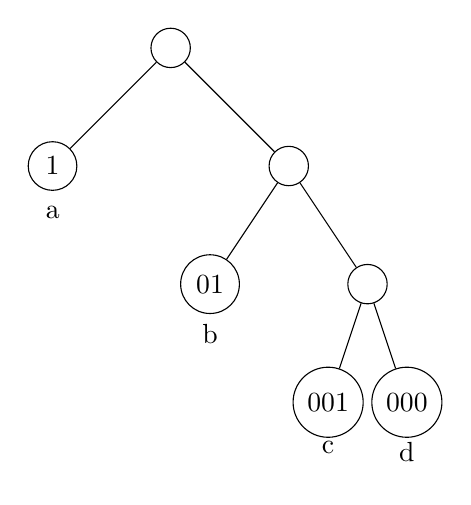
\begin{tikzpicture}[
            level distance=1.5cm,
            level 1/.style={sibling distance=3cm},
            level 2/.style={sibling distance=2cm},
            level 3/.style={sibling distance=1cm},
            every node/.style={circle,draw,minimum size=0.5cm},
            leaf label/.style={draw=none, circle=false, below=0.3cm}
        ]
            \node {}
                child {
                    node {1} 
                    node[leaf label] {a}
                }
                child {
                    node {}
                    child {
                        node {01}
                        node[leaf label] {b}
                    }
                    child {
                        node {}
                        child {
                            node {001}
                            node[leaf label] {c}
                        }
                        child {
                            node {000}
                            node[leaf label] {d}
                        }
                    }
                };
        \end{tikzpicture}
      \end{enumerate}
    \end{example}

    \begin{definition}[Prefix Code]
      Note that all of these encodings except for the nonvalid scheme has the property that no encoding of a character is a prefix of another character. A scheme with this property is called a \textbf{prefix code}. 
    \end{definition}

    \begin{example}
      By modifying the best scheme so far by swapping the $0$s and $1$s, we have 
        \begin{equation}
          C (s) = \begin{cases} 1 & s = a \\ 10 & s = b \\ 100 & s = c \\ 000 & s = d \end{cases}
        \end{equation}
        But this is not a prefix code, though it is a valid code (uniquely decodable since its symmetric counterpart is uniquely decodable). For example, we can sequentially decode the string 
        \begin{equation}
          1000000\ldots 
        \end{equation}
        since we don't know where the $0$s end. While we may be able to decode this if we knew the length, it isn't really easy to decode. 
    \end{example}

    The right intuition as this point is to give characters with large probabilities a short codeword and low ones longer ones. However, this is also not true. 

    \begin{example}
      Let's have the same alphabet but now slightly perturb the probabilities 
      \begin{equation}
        \mathbb{P}(a) = \frac{1}{4} + \epsilon,
        \mathbb{P}(b) = \frac{1}{4} + \frac{\epsilon}{2},
        \mathbb{P}(c) = \frac{1}{4} - \frac{\epsilon}{2},
        \mathbb{P}(d) = \frac{1}{4} - \epsilon,
      \end{equation}
      Then our prefix coding would be 
      \begin{equation}
        C (s) = \begin{cases} 1 & s = a \\ 01 & s = b \\ 001 & s = c \\ 000 & s = d \end{cases}
      \end{equation}
      which still has an expected length of $2.25$, which is not enough to beat just the regular 2-bit encoding of each word. 
    \end{example}

    Here is a better system of thinking about this. If all codewords have length $l$, then the number of codewords that we can make is $2^l$. Then we can think of each codeword of length $l$ having a ``cost'' of $2^{-l}$ in our \textit{codeword supermarket}. 

    \begin{figure}[H]
      \centering 
      \includegraphics[scale=0.4]{img/supermarket.png}
      \caption{Our symbol code supermarket where we can buy code words of length $l$ for a price of $2^{-l}$. Our budget is $1$. } 
      \label{fig:supermarket}
    \end{figure}

    With this visual, there are two constraints that we can reintroduce. First is Kraft's inequality. 

    \begin{theorem}[Kraft Inequality]
      Every viable symbol code must have a budget $\leq 1$. 
      \begin{equation}
        \sum_i 2^{-l_i} \leq 1
      \end{equation}
      If a symbol code achieves equality, then this is called a \textbf{complete symbol code}. 
    \end{theorem}

    Second, a prefix code must have all codewords in different ``rows'' of the supermarket. 

    \begin{figure}[H]
      \centering 
      \includegraphics[scale=0.4]{img/supermarket_prefix.png}
      \caption{A symbol code that is a prefix code. } 
      \label{fig:supermarket_prefix}
    \end{figure}

  \subsection{Huffman Coding}

    Now how well can we do with symbol codes? It turns out that the expected symbol code length cannot beat the entropy, and we will describe how to construct such a symbol code. 

    \begin{theorem}[Ideal Code Lengths]
      Given the expected length of a symbol code $C$ on an ensemble $X$, the expected length cannot be less than the entropy. 
      \begin{equation}
        H(X) \leq \mathbb{E}[\ell(C(X))] = \sum_{s \in \mathcal{S}} \mathbb{P}(s) l_i
      \end{equation}
    \end{theorem}
    \begin{proof}
      Such a code must exist. We first define the \textit{ideal length} of the character $s_i$ with probability $p_i$ to be its surprisal 
      \begin{equation}
        l_i^\ast = \log_2 \frac{1}{p_i} = \sigma_i
      \end{equation}
      If you rearrange this and imagine someone that picked length $l_i$. We can pick an implicit probability $q_i$ satisfying the ideal length.  It is $q_i = 2^{-l_i}$, but the person may not have chosen a complete code, so we must normalize it. 
      \begin{equation}
        q_i = \frac{2^{-l_i}}{Z}
      \end{equation}
      where $Z = 1$ if we have a complete code and $Z < 1$ if not. Therefore, we have 
      \begin{equation}
        l_i = \log_2 \frac{1}{q_i} - \log_2 Z 
      \end{equation}
      We can then plug this into the expected length formula. 
      \begin{align*}
        \mathbb{E}[\ell(C(X))] & = \sum_i p_i \bigg[ \log_2 \frac{1}{q_i} - \log_2 Z \bigg] \\
                               & = \sum_i p_i \log_2 \frac{1}{p_i} + \sum_i p_i \log_2 \frac{p_i}{q_i} - \log_2 Z \\
                               & = H(X) + D_{\mathrm{KL}} (p \mid \mid q) - \log Z \\
                               & \geq H(X)
      \end{align*}
      since the KL divergence (as we will show later) is greater than $0$, and since $Z \leq 1$, we are subtracting a negative number. 
    \end{proof}

    To get equality, the proof shows you that you must make your implicit probabilities equal to your true probabilities, so the length of each character should be equal to its surprisal or information content. But these lengths aren't integers, so we must modify this in practice, which will get close, but not exactly to the true minimum. It turns out that we can get the expected length $L$ such that it is within 1 bit of the true minimum. 
    \begin{equation}
      H(X) \leq L \leq H(X) + 1
    \end{equation}

    This is called the \textit{Huffman algorithm}. 

    \begin{theorem}[Huffman Algorithm]
      The \textbf{Huffman algorithm} constructs an optimal prefix code for a given set of symbols and their probabilities. The algorithm proceeds as follows:

      \begin{enumerate}
        \item Create a leaf node for each symbol, and add it to a priority queue.
        \item While there is more than one node in the queue:
        \begin{enumerate}
          \item Remove the two nodes with the lowest probability from the queue.
          \item Create a new internal node with these two nodes as children, with a probability equal to the sum of their probabilities.
          \item Add the new node back into the queue.
        \end{enumerate}
        \item The remaining node is the root of the Huffman tree.
        \item Traverse the tree, assigning 0 to each left branch and 1 to each right branch.
        \item The Huffman code for each symbol is the sequence of 0s and 1s on the path from the root to that symbol's leaf node.
      \end{enumerate}

      The Huffman algorithm produces an optimal prefix code, meaning that for any given set of symbols and probabilities, no other prefix code produces a smaller expected codeword length.
      \begin{enumerate}
        \item The expected length $L$ of the Huffman code satisfies:
        \begin{equation}
          H(X) \leq L < H(X) + 1
        \end{equation}
        \item The Huffman code is optimal among all prefix codes.
        \item Symbols with higher probabilities get shorter codewords.
        \item The algorithm has a time complexity of $O(n \log n)$ where $n$ is the number of symbols.
      \end{enumerate}
    \end{theorem}

    \begin{example}[Huffman Coding]
      Consider the alphabet $\mathcal{S} = \{A, B, C, D\}$ with probabilities $\{0.4, 0.3, 0.2, 0.1\}$.

      \begin{enumerate}
        \item Initial nodes: A(0.4), B(0.3), C(0.2), D(0.1)
        \item Combine D and C: (D,C)(0.3), A(0.4), B(0.3)
        \item Combine (D,C) and B: ((D,C),B)(0.6), A(0.4)
        \item Final tree: (A,((D,C),B))(1.0)
      \end{enumerate}

      \begin{figure}[H]
        \centering
        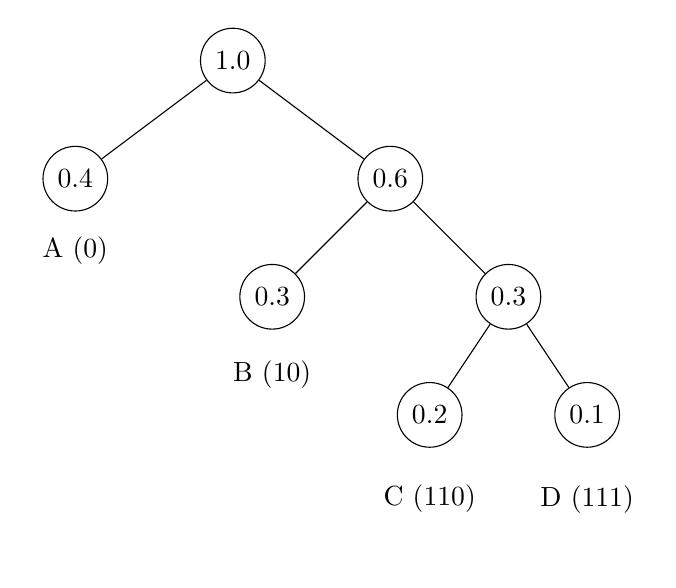
\begin{tikzpicture}[
          level distance=1.5cm,
          level 1/.style={sibling distance=4cm},
          level 2/.style={sibling distance=3cm},
          level 3/.style={sibling distance=2cm},
          every node/.style={circle,draw,minimum size=0.8cm},
          leaf label/.style={draw=none, circle=false, below=0.3cm}
        ]
          \node {1.0}
            child {
              node {0.4} 
              node[leaf label] {A (0)}
            }
            child {
              node {0.6}
              child {
                node {0.3}
                node[leaf label] {B (10)}
              }
              child {
                node {0.3}
                child {
                  node {0.2}
                  node[leaf label] {C (110)}
                }
                child {
                  node {0.1}
                  node[leaf label] {D (111)}
                }
              }
            };
        \end{tikzpicture}
        \caption{Huffman tree for the alphabet $\{A, B, C, D\}$}
        \label{fig:huffman_tree}
      \end{figure}

      Resulting codes:
      \begin{itemize}
        \item A: 0
        \item B: 10
        \item C: 110
        \item D: 111
      \end{itemize}

      The expected length is $L = 0.4(1) + 0.3(2) + 0.2(3) + 0.1(3) = 1.9$ bits compared to the entropy of $H(X) = -\sum_{i} p_i \log_2 p_i \approx 1.85$ bits. This demonstrates that the Huffman code achieves a length very close to the entropy, and always within 1 bit of it:
      \begin{equation}
        H(X) \approx 1.85 \leq L = 1.9 < H(X) + 1 \approx 2.85
      \end{equation}
    \end{example}

  \subsection{Lempel-Ziv (LZ) Compression}

    The \textbf{LZ77} and \textbf{LZ78} (also known as the \textbf{LZ1} and \textbf{LZ2}), respectively, are lossless data compression algorithms published by Lempel and Ziv in 1977/78. They obsolete themselves but form the basis for many modern variations including \textbf{LZW, LZSS, LZMA}, and others. 

    LZ77 and 78 are both dictionary coders, but are not static. Rather, the dictionary starts in some predetermined state but the contents change during the encoding process. 

\section{Differential Entropy}

  \subsection{Differential Entropy}

    \begin{definition}[Differential Entropy]
      For a continuous random vector, the \textbf{differential entropy} is defined 
      \begin{equation}
        H[\mathbf{X}] = - \int p(\mathbf{x}) \ln{p(\mathbf{x})} \,d\mathbf{x}
      \end{equation}
    \end{definition}

  \subsection{Kullback Leibler Divergence}

    The \textbf{relative entropy}, or \textbf{Kullback-Leibler divergence}, of distributions $p(x)$ and $q(x)$ is defined 
    \begin{align*}
      \mathrm{KL}(p || q) & \coloneqq - \int p(\mathbf{x}) \, \ln{q(\mathbf{x})} \,d\mathbf{x} - \bigg( - \int p(\mathbf{x}) \, \ln{p(\mathbf{x})} \,d\mathbf{x} \bigg) \\
      & = - \int p(\mathbf{x}) \, \ln \bigg( \frac{q(\mathbf{x})}{p(\mathbf{x})} \bigg) \,d\mathbf{x} 
    \end{align*}
    We can show that this quantity is always greater than or equal $0$ by Jensen's inequality using the fact that $-\ln(x)$ is concave
    \begin{equation}
      \int p(\mathbf{x}) \, -\ln \bigg( \frac{q(\mathbf{x})}{p(\mathbf{x})} \bigg) \,d\mathbf{x} \geq -\ln \int p(\mathbf{x}) \, \frac{q(\mathbf{x})}{p(\mathbf{x})} \,d\mathbf{x} = -\ln \int q(\mathbf{x}) \,d\mathbf{x} = -\ln(1) = 0
    \end{equation}
    and it is precisely $0$ if $p = q$, so it behaves similarly to a metric. However, it isn't exactly since it is not symmetric. 

    Let's demonstrate how entropy and the KL divergence applies to maximum likelihood estimation. Suppose that iid samples $\mathcal{D} = \{(x^{(n)}, y^{(n)}\}$ are given in a regression problem. Let $P^\ast = (X, Y)$ be the true data generating function. Then, we want to compute an approximation of $P^\ast$ with $P_\theta$, where $P_\theta$ is some parameterized distribution. The negative log likelihood of the $y$'s being generated is 
    \begin{equation}
      \ell(\theta) = \frac{1}{N} \sum_{n=1}^N \log P_\theta (y_i \mid x_i)
    \end{equation}
    which asymptotically converges to 
    \begin{equation}
      \mathbb{E}_{P^\ast} [ -\log P_\theta (y_i \mid x_i)] = \mathrm{KL}(P^\ast || P) + H[P^\ast]
    \end{equation}
    and since the entropy is constant, this is equivalent to minimizing the KL divergence between $P$ and $P^\ast$. 

    We assume that the $y^{(n)}$'s come from a conditional distribution $P_{\theta, x_i}$, where the parameters of the distribution is $\theta$ and $x_i$ 
  
  \subsection{Entropy of Probability Measures}

    First, we want to quantitatively measure the ``surprise'' of an event $E$ happening in a probability space by assigning it a value $H(E)$. We want it to satisfy the following: 
    \begin{enumerate}
      \item $H(E) \geq 0$. The surprisal of any event is nonnegative. 
      \item $H(E) = 0$ iff $\mathbb{P}(E) = 1$. No surprisal is gained from events with probability $1$. 
      \item If $E_1$ and $E_2$ are independent events, then $H(E_1 \cap E_2) = H(E_1) + H(E_2)$. The information from two independent events should be the sum of their informations. 
      \item $H$ should be continuous, i.e. slight changes in probability correspond to slight changes in surprisal. 
    \end{enumerate}

    \begin{definition}[Surprisal]
      Given a probability space $(\Omega, \mathcal{F}, \mathbb{P})$, the \textbf{surprisal}, or \textbf{self-information}, of an event $E \in \mathcal{F}$ is 
      \begin{equation}
        \sigma_\mathbb{P} (E) \coloneqq - \log \mathbb{P}(E)
      \end{equation}
      and the \textbf{expected surprisal} of $E$ is 
      \begin{equation}
        h_\mathbb{P} (E) = \mathbb{P}(E) \sigma_\mathbb{P} (E)
      \end{equation}
    \end{definition}

    Now we can define entropy as the expected surprisal of a random variable, which seems now more motivated and intuitive. 

    \begin{definition}[Entropy]
      Given a probability space $(\Omega, \mathcal{F}, \mathbb{P})$, a $\mathbb{P}$-almost partition is a set family $\mathcal{G} \subset \mathcal{F}$ such that $\mu(\cup_{G \in \mathcal{G}} G) = 1$ and $\mathbb{P}(A \cap B) = 0$ for all distinct $A, B \in \mathcal{G}$ (this is a relaxation of the usual conditions for a partition). The \textbf{entropy} of the subfamily $\mathcal{G}$ is 
      \begin{equation}
        H_\mathbb{P} (\mathcal{G}) \coloneqq \sum_{G \in \mathcal{G}} h_\mathbb{P}(G)
      \end{equation}
      The \textbf{entropy} of the $\sigma$-algebra $\mathcal{F}$ is defined 
      \begin{equation}
        H_\mathbb{P} (\mathcal{F}) = \sup_{\mathcal{G} \subset \mathcal{F}} H_\mathbb{P} (\mathcal{G})
      \end{equation}
      Now the entropy of a random variable $X: (\Omega, \mathcal{F}, \mathbb{P}) \rightarrow (\mathcal{X}, \mathcal{H})$ will induce a measure $\mathbb{P}_X$ on $\mathcal{X}$. Then the entropy of $X$ is defined over this induced measure. 
      \begin{equation}
        H[X] \coloneqq H_{\mathbb{P}_{X}} (\mathcal{H}) = \sup_{G \subset \mathcal{H}} H_{\mathbb{P}_X} (\mathcal{G})
      \end{equation}
    \end{definition}

    Intuitively, this represents the element of surprise of a certain data point, and distributions that have relatively sharp peaks will have lower entropy (since we expect most of the samples to come from the peaks) while uniform distributions have higher entropy. 

\section{Relative Entropy and Mutual Information}

  Informally, the relative entropy is a measure of the distance between two distributions. That is, the relative entropy $D(p||q)$ is a measure of the inefficiency of assuming that the distribution is $q$ when the true distribution is $p$. For example, if we knew the true distribution $p$ of the random variable, we could construct a code with average description length $H(p$. If, instead, we used the code for a distribution $q$, we would need $H(p) + D(p||q)$ bits on the average to describe the random variable. 

  \begin{definition}[Kullback-Leibler Divergence]
  The \textbf{relative entropy}, or \textbf{Kullback-Leibler distance}, between two probability mass functions $p(x)$ and $q(x)$ is defined as 
  \begin{align*}
      D(p||q) & = \sum_{x \in \mathcal{X}} p(x) \, \log \frac{p(x)}{q(x)} \\
      & = \mathbb{E}_p \bigg( \log \frac{p(X)}{q(X)} \bigg)
  \end{align*}
  In other words, it is the expectation of the logarithmic difference between the probabilities $P$ and $Q$, where the expectation is taken using the probabilities $P$. It is a measure of how one probability distribution is different from a second, reference probability distribution. A relative entropy of $0$ indicates that $p$ and $q$ are identical. It is useful to interpret this measure as a "distance" between two distributions, but it is not a formal metric because it is not symmetric 
  \[D(p||q) = \mathbb{E}_p \bigg( \log \frac{p(X)}{q(X)} \bigg) \neq \mathbb{E}_q \bigg( \log \frac{q(X)}{p(X)} \bigg) = D(q||p)\]
  and does not satisfy the triangle inequality. 
  \end{definition}

  \begin{definition}
  Consider two random variables $X$ and $Y$ with a joint probability mass function $p(x, y)$ and marginal probability mass functions $p(x)$ and $p(y)$. The \textbf{mutual information} $I(X; Y)$ is the relative entropy between the joint distribution and product distribution $p(x) p(y)$. 
  \begin{align*}
      I(X;Y) & = \sum_{x \in \mathcal{X}} \sum_{y \in \mathcal{Y}} p(x, y)\, \log \frac{p(x, y)}{p(x) p(y)} \\
      & = D\big( p(x, y)||p(x) p(y)\big) \\
      & = \mathbb{E}_{p(x, y)} \bigg( \log \frac{p(X, Y)}{p(X) p(Y)} \bigg)
  \end{align*}
  \end{definition}

  \begin{theorem}[Mutual Information and Entropy]
  The mutual information $I(X;Y)$ is the reduction in the uncertainty of $X$ due to the knowledge of $Y$. 
  \[I(X;Y) = H(X) - H(X|Y)\]
  It follows that
  \begin{align*}
      I(X;Y) & = H(X) - H(X|Y) \\
      & = H(Y) - H(Y|X) \\
      & = H(X) + H(Y) - H(X, Y) \\
      I(X;Y) & = I(Y;X) \\
      I(X;X) & = H(X)
  \end{align*}
  We can visualize it as such: 
  \begin{center}
  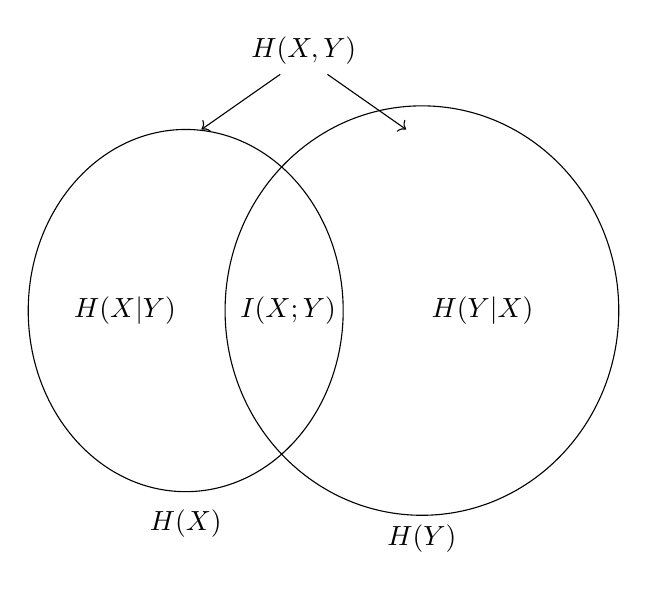
\begin{tikzpicture}
      \draw (-1.5, 0) ellipse (2 and 2.3);
      \draw (1.5, 0) ellipse (2.5 and 2.6);
      \node[left] at (-1.5,0) {$H(X|Y)$};
      \node[right] at (1.5,0) {$H(Y|X)$};
      \node[below] at (-1.5, -2.4) {$H(X)$};
      \node[below] at (1.5, -2.6) {$H(Y)$};
      \node at (-0.2, 0) {$I(X;Y)$};
      \draw[->] (-0.3, 3)--(-1.3, 2.3);
      \draw[->] (0.3,3)--(1.3, 2.3);
      \node[above] at (0,3) {$H(X, Y)$};
  \end{tikzpicture}
  \end{center}
  \end{theorem}
  \begin{proof}
  We can write
  \begin{align*}
      I(X;Y) & = \sum_{x, y} p(x, y) \, \log \frac{p(x, y)}{p(x)p(y)} \\
      & = \sum_{x, y} p(x, y) \log \frac{p(x|y)}{p(x)} \\
      & = - \sum_{x, y} p(x, y) \log p(x) + \sum_{x, y} p(x, y) \log p(x|y) \\
      & = - \sum_x p(x) \log p(x) - \Bigg( - \sum_{x, y} p(x, y) \log p(x|y) \Bigg) \\
      & = H(X) - H(X|Y)
  \end{align*}
  By symmetry, we have
  \[I(X;Y) = H(Y) - H(Y|X)\]
  Thus, $X$ says as much about $Y$ as $Y$ says about $X$. Since $H(X, Y) = H(X) + H(Y|X)$, we have
  \[I(X;Y) = H(X) + H(Y) - H(X, Y) \implies I(X;X) = H(X) - H(X|X) = H(X)\]
  That is, the mutual information of a random variable with itself is the entropy of the random variable. This is the reason that entropy is sometimes referred to as \textit{self-information}. 
  \end{proof}

  \begin{example}
  For the joint distribution in the previous example, the mutual information is 
  \[I(X;Y) = H(Y) - H(Y|X) = 2 - \frac{13}{8} = \frac{3}{8} \text{ bits}\]
  \end{example}

  \begin{definition}
  The \textbf{conditional mutual information} of random variables $X, Y, Z$ is the reduction in the uncertainty of $X$ due to knowledge of $Y$ when $Z$ is given. 
  \begin{align*}
      I(X;Y|Z) & = H(X|Z) - H(X|Y, Z) \\
      & = E_{p(x, y, z)} \bigg( \log \frac{p(X, Y|Z)}{p(X|Z) p(Y|Z)}\bigg)
  \end{align*}
  \end{definition}

  Mutual information also satisfies a chain rule. 

  \begin{theorem}[Chain rule for information]
  \[I(X_1, X_2, ..., X_n; Y) = \sum_{i=1}^n I(X_i;Y|X_{i-1}, ..., X_1)\]
  \end{theorem}
  \begin{proof}
  \begin{align*}
      I(X_1, ..., X_n;Y) & = H(X_1, ..., X_n) - H(X_1, ..., X_n |Y) \\
      & = \sum_{i=1}^n H(X_i|X_{i-1}, ..., X_1) - \sum_{i=1}^n H(X_i | X_{i-1}, ..., X_1;Y) \\
      & = \sum_{i=1}^n I(X_i ; Y|X_1, X_2, ..., X_{i-1})
  \end{align*}
  \end{proof}

  We now define a conditional version of relative entropy.

  \begin{definition}
  For joint probability mass functions $p(x, y)$ and $q(x, y)$, the \textbf{conditional relative entropy} $D\big( p(y|x) || q(y|x)\big)$ is the average of the relative entropies between the conditional probability mass functions $p(y|x)$ and $q(y|x)$ averaged over the probability mass function $p(x)$. That is, 
  \begin{align*}
      D\big(p(y|x)||q(y|x)\big) & = \sum_x p(x) \sum_y p(y|x) \, \log \frac{p(y|x)}{q(y|x)} \\
      & = \mathbb{E}_{p(x, y)} \bigg( \log \frac{p(Y|X)}{q(Y|X)} \bigg) 
  \end{align*}
  \end{definition}

  \subsection{Information Content}
  The \textbf{information content, self-information, surprisal}, or \textbf{Shannon information}, is a basic quantity derived from the probability of a particular event occurring from a random variable. It can be thought of as an alternative way of expressing probability, much like odds or log-odds, but which has particular mathematical advantages in the setting of information theory. The self-information can be interpreted as quantifying the level of "surprise" of a particular outcome. The information content can be expressed in various units of information, of which the most common is the "bit" (sometimes also called the \textit{shannon}), as explained below. 

  The definition of self-information was chosen to meet several axioms: 
  \begin{enumerate}
      \item An event with probability 100\% is perfectly unsurprising and yields no information.
      \item The less probable an event is, the more surprising it is and the more information it yields.
      \item If two independent events are measured separately, the total amount of information is the sum of the self-informations of the individual events. 
  \end{enumerate}
  It can be shown that there is a unique function of probability that meets these three axioms, up to a multiplicative scaling factor. Broadly given an event $x$ with probability $P$, the information content is defined as follows: 
  \[I(x) \equiv - \log_b \big( \mathbb{P}(x)\big)\]
  The base of the log is left unspecified, which corresponds to the scaling factor above. Formally, given a continuous random variable $X$ with probability density function $p_X (x)$, the self-information of measuring $X$ as outcome $x$ is defined as:
  \[I_X (x) \equiv - \log \big( p_X (x) \big) = \log \bigg(\frac{1}{p_X (x)}\bigg)\]

  \subsubsection{Properties}
  For a given probability space, the measurement of rarer events are intuitively more "surprising," and yield more information content, than more common values. Thus, self-information is a strictly decreasing monotonic function of the probability. While standard probabilities are represented by real numbers in the interval $[0,1]$, self-informations are represented by extended real numbers in the interval $[0,\infty]$. In particular, we have the following, for any choice of logarithmic base:
  \begin{enumerate}
      \item If a particular event has a 100\% probability of occurring, then its self-information is $-\log (1) = 0$: its occurrence is \textit{perfectly non-surprising} and yields no information.
      \item If a particular event has a 0\% probability of occurring, then its self-information is $- \log (0) = \infty$: its occurrence is \textit{infinitely surprising}.
  \end{enumerate}
  From this, we can get a few general properties: 
  \begin{enumerate}
      \item Intuitively, more information is gained from observing an unexpected event—it is \textit{surprising}.
      \item This establishes an implicit relationship between the self-information of a random variable and its variance. 
  \end{enumerate}
  Note also that this definition of information content satisfies additivity. Consider two independent random variables $X, Y$ with probability mass functions $p_X (x)$ and $p_Y (y)$ respectively. The joint probability mass function is 
  \[p_{X, Y} (x, y) \equiv \mathbb{P} (X = x, Y = y) = p_X (x) \, p_Y (y)\]
  because $X$ and $Y$ are independent. The information content of the outcome $(X, Y) = (x, y)$ is 
  \begin{align*}
      I_{X, Y} (x, y) & = - \log_2 \big( p_{X, Y} (x, y) \big) ]\\
      & = -\log_2 \big(p_X (x) \, p_Y (y)\big) \\
      & = - \log_2 \big( p_X (x) \big) - \log_2 \big( p_Y (y) \big) \\
      & = I_X (x) + I_Y (y)
  \end{align*}

  A fair coin toss, which can be measured by the Bernoulli distribution $\mathbb{P}(H) = \frac{1}{2}, \;\; \mathbb{P}(T) = \frac{1}{2}$ has the information contents (in bits, base 2) 
  \begin{align*}
      I_X (H) & = - \log_2 \big( \mathbb{P}(X = H)\big) = - \log_2 \frac{1}{2} = 1 
      I_X (T) & = - \log_2 \big( \mathbb{P}(X = T)\big) = - \log_2 \frac{1}{2} = 1 
  \end{align*}
  A fair six-sided die roll has the discrete uniform distribution. The information content is 
  \[I_X (1) = I_X (2) = I_X (3) = I_X (4) = I_X (5) = I_X (6) = -\log_2 \frac{1}{6} \approx 2.585\]
  Two independent, identically distributed dice gives an information content of 
  \[I_{X, Y} (x, y) = -\log_2 \frac{1}{36} \approx 5.169925\]
  where $1 \leq x, y \leq 6$. Note that this could have also been calculated by simply adding the self-information of one die with that of another identical die.

  \subsection{Entropy}
  The \textbf{entropy} of a random variable is the average level of \textit{information}, \textit{surprise}, or \textit{uncertainty} inherent in the variable's possible outcomes. As an example, consider a biased coin with probability p of landing on heads and probability 1-p of landing on tails. The maximum surprise is for p = 1/2, when there is no reason to expect one outcome over another, and in this case a coin flip has an entropy of one bit. The minimum surprise is when p = 0 or p = 1, when the event is known and the entropy is zero bits. Other values of p give different entropies between zero and one bits.

  Given a discrete random variable $X$, with possible outcomes $x_1, x_2, ..., x_n$ which occur with probability $P(x_1), P(x_2), ..., P(x_n)$, the entropy of $X$ is formally defined as: 
  \begin{align*}
      H(X) & \equiv - \sum_{i=1}^n \mathbb{P}(x_i) \, \log \mathbb{P}(x_i) \\
      & \equiv \mathbb{E}\big(I_X (X)\big)
  \end{align*}
  which is the expected information content of measurement of $X$. Base 2 gives the unit of bits, while base $e$ gives the \textit{natural units} nat, and base 10 gives a unit called dits. 

  The entropy was originally created by Shannon as part of his theory of communication, in which a data communication system is composed of three elements: a source of data, a communication channel, and a receiver. In Shannon's theory, the "fundamental problem of communication" – as expressed by Shannon – is for the receiver to be able to identify what data was generated by the source, based on the signal it receives through the channel. Shannon considered various ways to encode, compress, and transmit messages from a data source, and proved in his famous source coding theorem that the entropy represents an absolute mathematical limit on how well data from the source can be losslessly compressed onto a perfectly noiseless channel. 

  The English text, treated as a string of character, has fairly low entropy, i.e. is fairly predictable. If we do not know exactly what is going to come next, we can be fairly certain that, for example, 'e' will be far more common than 'z', that the combination 'qu' will be much more common than any other combination with a 'q' in it, and that the combination 'th' will be more common than 'z', 'q', or 'qu'. After the first few letters one can often guess the rest of the word. English text has between 0.6 and 1.3 bits of entropy per character of the message. 

  \subsubsection{Shannon's Source Coding Theorem}
  If a compression scheme is lossless – one in which you can always recover the entire original message by decompression – then a compressed message has the same quantity of information as the original, but communicated in fewer characters. It has more information (higher entropy) per character. A compressed message has less redundancy. Shannon's source coding theorem states a lossless compression scheme cannot compress messages, on average, to have more than one bit of information per bit of message, but that any value less than one bit of information per bit of message can be attained by employing a suitable coding scheme. The entropy of a message per bit multiplied by the length of that message is a measure of how much total information the message contains.

  This theorem establishes the limits to possible data compression. Informally, it states that 
  \begin{center}
      $N$ i.i.d. random variables each with entropy $H(X)$ can be compressed into more than $N$ $H(X)$ bits with negligible risk of information loss, as $N \rightarrow \infty$; but conversely, if they are compressed into fewer than $N$ $H(X)$ bits, it is virtually certain that information will be lost. 
  \end{center}

\section{Data Compression}

  \textbf{Data compression}, also called \textbf{source coding} or  \textbf{bit-rate reduction}, is the process of encoding information using fewer bits than the original representation. Data compression algorithms can be categorzied into two types: 
  \begin{enumerate}
      \item \textbf{Lossless compression} reduces bits by identifying and eliminating statistical redundancy. No information is lost in lossless compression. 
      \item \textbf{Lossy compression} reduces bits by removing unnecessary or less important information.
  \end{enumerate}
  Typically, a device that performs data compression is referred to as an \textbf{encoder}, and one that performs the reversal of the process (decompression) as a \textbf{decoder}. 

  A \textbf{space–time} or \textbf{time–memory trade-off} in computer science is a case where an algorithm or program trades increased space usage with decreased time. Here, space refers to the data storage consumed in performing a given task (RAM, HDD, etc), and time refers to the time consumed in performing a given task (computation time or response time). 

  A space–time trade-off can be applied to the problem of data storage. If data is stored uncompressed, it takes more space but access takes less time than if the data were stored compressed (since compressing the data reduces the amount of space it takes, but it takes time to run the decompression algorithm). Depending on the particular instance of the problem, either way is practical. There are also rare instances where it is possible to directly work (which may also be faster) with compressed data. 

  \subsection{Data Compression Ratio}
  The \textbf{data compression ratio}, also known as the \textbf{compression power}, is a measurement of the relative reduction in size of data representation produced by a data compression algorithm. It is defined as 
  \[\text{Compression Ratio} = \frac{\text{Uncompressed Size}}{\text{Compressed Size}}\]
  For example, a representation that compresses a file's storage size from 10MB to 2MB has a compression ratio of $10/2 = 5$. We can alternatively talk about the \textbf{space saving}, which is defined
  \[\text{Space Saving} = 1 - \frac{\text{Compressed Size}}{\text{Uncompressed Size}}\]
  So, the previous representation yields a space saving of 0.8, or $80\%$. 

  Lossless compression of digitized data such as video, digitized film, and audio preserves all the information, but it does not generally achieve compression ratio much better than 2:1 because of the \textbf{intrinsic entropy} of the data. Compression algorithms which provide higher ratios either incur very large overheads or work only for specific data sequences (e.g. compressing a file with mostly zeros). In contrast, lossy compression (e.g. JPEG for images, or MP3 and Opus for audio) can achieve much higher compression ratios at the cost of a decrease in quality, such as Bluetooth audio streaming, as visual or audio compression artifacts from loss of important information are introduced. In general, whether a compression ratio is high or not really depends on what kind of data is being compressed and how it is compressed. 


  \subsection{Lossless Compression}
  Lossless data compression algorithms usually exploit statistical redundancy to represent data without losing any information, so that the process is reversible. Lossless compression is possible because most real-world data exhibits statistical redundancy. For example, an image may have areas of color that do not change over several pixels; instead of coding "red pixel, red pixel, ..." the data may be encoded as "279 red pixels". This is a basic example of run-length encoding; there are many schemes to reduce file size by eliminating redundancy.

  A \textbf{dictionary coder}, also known as a \textbf{substitution coder}, is a class of lossless data compression algorithms which operate by searching for matches between the text to be compressed and a set of strings contained in a data structure (called the 'dictionary') maintained by the encoder. When the encoder finds such a match, it substitutes a reference to the string's position in the data structure. 

  Some dictionary coders use a \textit{static dictionary}, one whose full set of strings is determined before coding begins and does not change during the coding process. This approach is most often used when the message or set of messages to be encoded is fixed and large; for instance, an application that stores the contents of a book in the limited storage space of a PDA generally builds a static dictionary from a concordance of the text and then uses that dictionary to compress the verses. 

  In a related and more general method, a dictionary is built from redundancy extracted from a data environment (various input streams) which dictionary is then used statically to compress a further input stream. For example, a dictionary is built from old English texts then is used to compress a book. More common are methods where the dictionary starts in some predetermined state but the contents change during the encoding process, based on the data that has already been encoded. 

  \subsubsection{Run-length Encoding (RLE) Compression}
  RLE is a form of lossless data compression in which \textit{runs} of data (sequences in which the same data value occurs in many consecutive data elements) are stored as a single data value and count, rather than as the original run. This is most useful on data that contains many such runs.

  For example, consider a screen containing plain black text on a solid white background. There will be many long runs of white pixels in the blank space, and many short runs of black pixels within the text. A hypothetical scan line, with B representing a black pixel and W representing white, might read as follows: 
  \begin{lstlisting}
  WWWWWWWWWWWWBWWWWWWWWWWWWBBBWWWWWWWWWWWWWWWWWWWWWWWWBWWWWWWWWWWWWWW
  \end{lstlisting}
  With a RLE data compression algorithm applied to the above hypothetical scan line, it can be rendered as follows: 
  \begin{lstlisting}
  12W1B12W3B24W1B14W
  \end{lstlisting}
  which can be interpreted as a sequence of 12 Ws, 1 B, 12 Ws, 3 Bs, and so on. This run-length code represents the original 67 characters in only 18. While the actual format used for the storage of images is generally binary rather than ASCII characters like this, the principle remains the same. Even binary data files can be compressed with this method. 

\bibliographystyle{plain}
\bibliography{./bibfile}
\end{document}
